\documentclass[11pt,a4paper]{article}
\usepackage{amssymb} %mathbb
\usepackage{amsmath} %align
\usepackage{graphicx} %jpg
\usepackage{cancel}
\usepackage{hyperref} %a href
\usepackage{gensymb}
\usepackage{colortbl}
\usepackage{amsthm}
\newtheorem{exercise}{Exercise}
\newtheorem{definition}{Definition}
\newtheorem{thm}{Theorem}
\newtheorem{example}{Example}
\usepackage[top=1.0cm,bottom=1.3cm,left=1.0cm,right=1.0cm]{geometry}

\begin{document}

\section{Estudo da fun\c{c}\~ao $W$ de Lambert}

		\begin{center}
		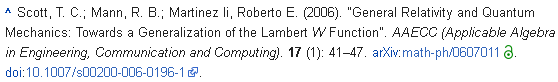
\includegraphics[scale=1]{referencia}
		\end{center}

\vspace{3mm}

Sabemos pelos poderes de Wolfram Alpha que:

\begin{align}
  e^{-cx} &= a (x - r) \Leftrightarrow x = \cfrac{W_n\left(\cfrac{c e^{-cr}}{a} \right) + cr}{c} \label{primeiro_grau}
\end{align}

\vspace{3mm}

O autor quer resolver a equa\c{c}\~ao

\begin{align}
  e^{-cx} &= a (x - r_1) (x - r_2) \\
  e^{-2xR} &= a_0 b_0 (x - r_1) (x - r_2)
\end{align}

\vspace{3mm}

Para isso, ele cria uma vari\'avel independente $y$, tal que vale a seguinte decomposi\c{c}\~ao:

\begin{align}
  e^{-Rxy} &= a_0 (x - r_1) \\
  e^{-Rx(2 - y)} &= b_0 (x - r_2)
\end{align}

Resolve cada uma delas fazendo $x = f(y)$ e usando a equa\c{c}\~ao (\underline{\color{blue}\ref{primeiro_grau}}).

\begin{align}
  x &= \cfrac{W_n(z_1) + Ryr_1}{Ry} \\
  x &= \cfrac{W_n(z_2) + R(2 - y)r_2}{R(2 - y)} \\
  z_1 &= \cfrac{yRe^{-r_1yR}}{a_0} \\
  z_2 &= \cfrac{(2-y)Re^{-r_2(2-y)R}}{b_0}
\end{align}

\vspace{3mm}

Como os \'ecses ou xizes s\~ao iguais, ficamos com a depend\^encia em $y$ abaixo. (N\~ao gostei do \'epsilon.)

A solu\c{c}\~ao em $x$ vai junto um pouquinho mais abaixo:

\begin{align}
  r_1 - r_2 &= \cfrac{W_n(z_2)}{(2-y)R} - \cfrac{W_n(z_1)}{yR} \\
  x &= - \cfrac{1}{2R}\, \ln \left[ a_0 b_0 \cfrac{W_n(z_1) W_n(z_2)}{y(2 - y)R^2} \right]
\end{align}

\vspace{3mm}

O resto do artigo \'e desnecess\'ario. O cara quer usar as propriedades abaixo:

\begin{align}
  W(z_1) W(z_2) &= z_1 z_2 e^{-W(z_1) - W(z_2)} \\
  W(z_1) + W(z_2) &= W \left( z_1 z_2 \left( \cfrac{1}{W(z_1)} + \cfrac{1}{W(z_2} \right) \right) \\
  \therefore 2xR &= W(z_1) + W(z_2) + r_1 y R + r_2 (2 - y) R
\end{align}

\vspace{100mm}

Antes de variar o grau, deixe-me registrar algumas tentativas.

\begin{align}
r_1 &= r_2 = r \\
\alpha &= r_1 - r_2 = 0 \\
e^{-xR} &= \pm \sqrt{a_0 b_0} \, (x - r) \\
x &= \cfrac{W(\pm Re^{-Rr}/\sqrt{a_0 b_0}) + Rr}{R} = \cfrac{W(\pm \lambda)}{R} + r = \cfrac{k}{R} + r = \cfrac{1}{2R}\, (w_1 + w_2 + 2rR) \\
\cfrac{w_2}{(2 - y)R} &= \cfrac{w_1}{yR} \Rightarrow w_2 = w_1\cdot \cfrac{2 - y}{y} \\
W(\pm \lambda) &= \cfrac{1}{2} \cdot w_1\cdot \bigg( 1 + \cfrac{2 - y}{y} \bigg) = \cfrac{w_1}{y} \\
w_1 &= ky \Rightarrow kye^{ky} = z_1 = \cfrac{yRe^{-rRy}}{a_0} \\
a_0 k \exp ( ky + rRy ) &= R \\
a_0 k \gamma^y &= R\,;\,\gamma = \exp ( k + rR ) \\
y &= \log_{\gamma} \bigg( \cfrac{R}{a_0 k} \bigg) = \cfrac{\ln R - \ln a_0 - \ln k}{k + rR}
\end{align}

Sem perda de generalidade, o pr\'oximo passo \'e $\alpha > 0$. Este caminho parece que vai dar em lugar nenhum.

\begin{align}
r_1 &= r \\
r_2 &= r - \alpha \\
w_2 &= w_1\cdot \cfrac{2 - y}{y} + \alpha (2 - y) R \\
x(y) &= \cfrac{1}{2R}\, \bigg[w_1\bigg(1 + \cfrac{2 - y}{y}\bigg) + \alpha (2 - y) R + ryR + (r - \alpha)(2 - y)R\bigg] \\
x &=  \cfrac{1}{2R}\,\,w_1\,\cfrac{2}{y} + r \text{ // mas } y \text{ depende de }\alpha\,!!! \\
w_1 &= (x - r)Ry \Rightarrow k = (x - r)R \Rightarrow y(x) = - \cfrac{\ln a_0 + \ln (x - r)}{xR} \\
x &=  \cfrac{w_2}{(2-y)R} + r - \alpha \\
w_2 &= (x - r + \alpha)R(2-y) \\
z_2 &= (x - r + \alpha)R(2-y)e^{(x - r)R(2-y)}e^{\alpha R(2-y)} = \cfrac{(2 - y)Re^{\alpha(2 - y)R}e^{-r(2 - y)R}}{b_0} \\
b_0 (x - r + \alpha)e^{xR(2-y)} &= 1 \\
xR(2-y) &= \ln 1 - \ln b_0 - \ln (x - r + \alpha) \\
xRy &= 2xR + \ln b_0 + \ln (x - r + \alpha) \\
y(x) &= 2 + \cfrac{\ln b_0 + \ln (x - r + \alpha)}{xR}
\end{align}

Terceiro grau! A partir de agora o Jo\~ao escritor do apocalipse, e ao mesmo tempo a Besta do apocalipse reencarnada, vamos escrever coisas \'obvias:

\begin{align}
  -2R &= \ln b\,;\,y \leftarrow 2y\,;\,u \leftarrow 2u \\
  b^x &= a (x - r_1) (x - r_2) (x - r_3) \\
  b^{xy} &= a (x - r_1) \\
  b^{xu} &= 1 (x - r_2) \\
  b^{x(1 - y - u)} &= 1 (x - r_3) \\
  -x \ln b &= \cfrac{W(z_1) - y r_1 \ln b}{y} = \cfrac{W(z_2) - u r_2 \ln b}{u} = \cfrac{W(z_3) - (1 - y - u) r_3 \ln b}{1 - y - u} \\
  F(y,u) &= (0,0) \\
  z_1 &= - \cfrac{yb^{r_1y} \ln b}{a} \\
  z_2 &= -u b^{r_2u} \ln b \\
  z_3 &= -(1-y-u) b^{r_3(1-y-u)} \ln b \\
  x &= \log_b \left[ -\cfrac{a}{(\ln b)^3} \cdot \cfrac{W(z_1)}{y} \cdot \cfrac{W(z_2)}{u} \cdot \cfrac{W(z_3)}{1 - y - u} \right] \\
  \therefore -x \ln b &= W(z_1) + W(z_2) + W(z_3) - r_1 y \cdot \ln b - r_2 u \cdot \ln b - r_3 (1 - y - u) \ln b
\end{align}

\vspace{3mm}

Mas n\~ao \'e s\'o isso.

\begin{align}
  e^{-2xR} &= a_0 (x - r_1) (x - r_2) (x - r_3) (x - r_4) \\
  e^{-Rxy} &= a_0 (x - r_1) \\
  e^{-Rxu} &= 1 (x - r_2) \\
  e^{-Rxv} &= 1 (x - r_3) \\
  e^{-Rx(2 - y - u - v)} &= 1 (x - r_4) \\
  x &= \cfrac{W(z_1) + Ry r_1}{Ry} = \cfrac{W(z_2) + Ru r_2}{Ru} = \cfrac{W(z_3) + Rv r_3}{Rv} = \cfrac{W(z_4) + R(2 - y - u - v) r_4}{R(2 - y - u - v)} \\
  F(y,u,v) &= (0,0,0) \\
  z_1 &= \cfrac{yRe^{-r_1yR}}{a_0} \\
  z_2 &= uRe^{-r_2uR} \\
  z_3 &= vRe^{-r_3vR} \\
  z_4 &= (2-y-u-v)Re^{-r_4(2-y-u-v)R} \\
  x &= - \cfrac{1}{2R}\, \ln \left[ a_0 \cdot \cfrac{W(z_1)}{Ry} \cdot \cfrac{W(z_2)}{Ru} \cdot \cfrac{W(z_3)}{Rv} \cdot \cfrac{W(z_4)}{R(2 - y - u - v)} \right] \\
  \therefore 2xR &= W(z_1) + W(z_2) + W(z_3) + W(z_4) + r_1 y R + r_2 u R + r_3 v R + r_4 (2 - y - u - v) R
\end{align}

\vspace{3mm}

Nossa tese \'e que a qu\'intica \'e sol\'uvel desta forma. Sempre que qualquer polin\^omio de grau $n$ entrar em jogo, este encantamento permite pela matriz companheira passar \`a exponencial, e remover do jogo instantaneamente aquele polin\^omio pela fun\c{c}\~ao $W$ de Lambert.

\vspace{3mm}

Out of charity, there is no salvation at all.

\vspace{3mm}

Vinicius Claudino FERRAZ, 30/May/2019

\end{document}
